\chapter{NGHDL: Mixed Signal Simulation}
\label{chap9}
\thispagestyle{empty}


NGHDL feature facilitates creation of user-defined models for mixed-signal circuit simulation in eSim. By interfacing GHDL and Ngspice, we achieve mixed-signal simulation. Digital models are simulated using GHDL and XSPICE engine of Ngspice. \\


%To access NGHDL click on the NGHDL button on the left pane of window as shown in figure \figref{screen3}:
%\pagebreak

\section{Introduction}

Ngspice supports mixed-signal simulation, i.e. it can simulate both digital and analog component. It defines a \texttt{model} which has the functionality of the circuit component, which can be used in the netlist.
For example you can create an \texttt{adder} model in Ngspice and use it in any circuit netlist of Ngspice. \\

However, it is not feasible to define complex digital models without a complete understanding of Ngspice and XSPICE architectures and is a time-consuming process. Also, most of the users are familiar with GHDL and can write the models using VHDL code with ease.
Hence, NGHDL provides an  interface to write VHDL code for a digital model and install it as model in Ngspice. So whenever Ngspice looks for that model, it will actually interface with VHDL code to get the result. \\

\begin{figure}[!htp]
\centering
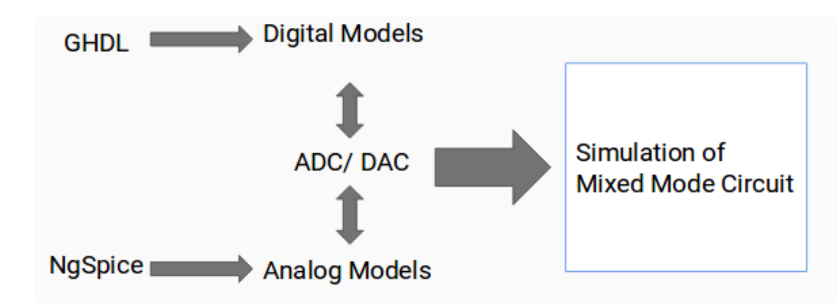
\includegraphics[width = 13cm, height = 7cm]{./NGHDL/NGHDL_Overview.png}
\caption{Overview of NGHDL}
\label{overview}
\end{figure}
%description of Overview:
\figref{overview} shows the overview of NGHDL indicating its architecture at the abstract level. The values for the digital models present in the netlist are fetched from the GHDL side of the interface whereas the values of the analog part are fetched from Ngspice's spice3f5 engine. Digital and Analog components in \figref{overview} are connected to each other with the help of the hybrid ADC and DAC models provided by Ngspice. This helps in the signal level switching when simulation is performed. As analog signals are in continuous time domain and Digital signals are in discrete time domain, hybrid components help bridge the gap. More information on the parameters of ADC and DAC present in Appendix : D.

\pagebreak

\section{Digital Model creation using NGHDL}

%Description of User Flow of NGHDL

\begin{figure}[!htp]
\centering
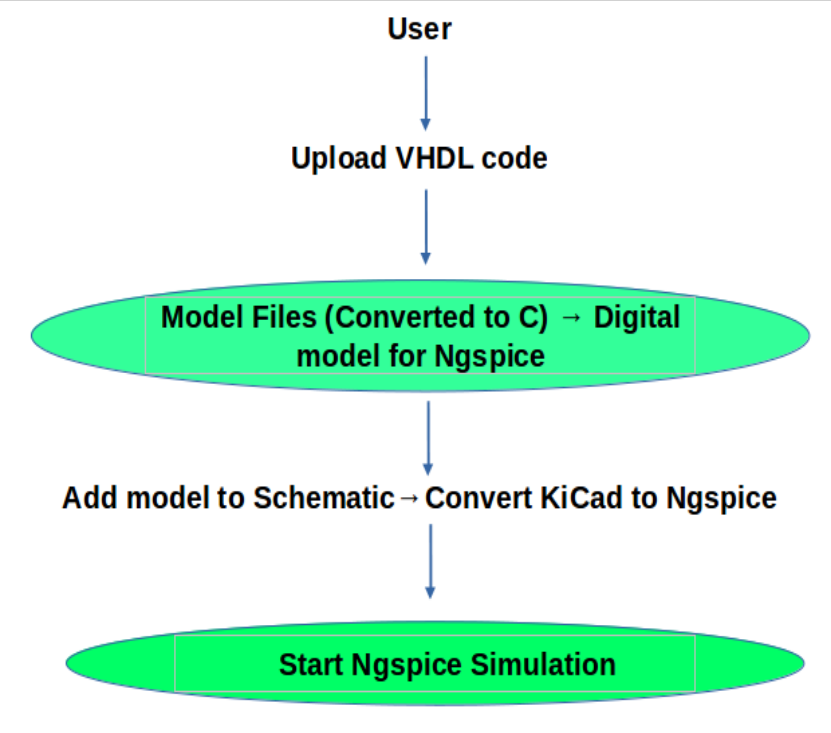
\includegraphics[width = 13cm, height = 7cm]{./NGHDL/NGHDL_Flow.png}
\caption{User Flow for NGHDL}
\label{user_flow}
\end{figure}

\noindent \textbf{The steps to create digital models are given below}:

\begin{enumerate}
\item Click on NGHDL button on left side pane of main window, the Ngspice Digital Model Creator window will appear as shown in  \figref{screen3}
        \begin{figure}[!htp]
            \centering
            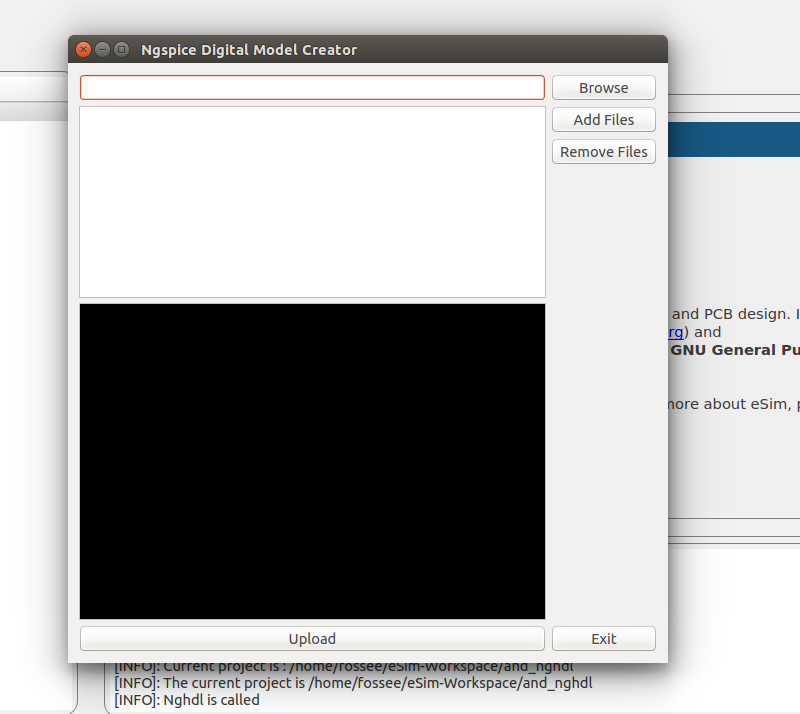
\includegraphics[height=10cm, width =\lgfig]{./NGHDL/screen3.png}
            \caption{NGHDL interface}
            \label{screen3}
        \end{figure}


\item Now browse and locate the VHDL file to upload. Select the VHDL file and click on the Upload button. This process will create Ngspice model and corresponding component drawing inside the KiCad library (eSim\_Nghdl.lib) of the VHDL block to be used in mixed-signal simulations. An acknowledgement message will appear upon sucessful processing of the VHDL code as shown in \figref{upload}. \\

        \begin{figure}[!htp]
            \centering
            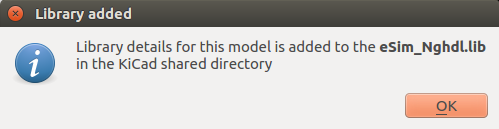
\includegraphics[width =\smfig]{./NGHDL/screen4.png}
            \caption{Uploading of digital model}
            \label{upload}
         \end{figure}
         
Note : \texttt{"Add files"} option allow you to use a smaller entity / subpart / submodule to support the main VHDL file. That is, a digital model will be generated corresponding to that file that has been browsed. The file that has been \texttt{"added"} to Nghdl upload window will only be placed along with the model under model’s DUTghdl folder to support the model.

Hence, \texttt{"browsing"} one file and \texttt{"adding"} several files won’t create that many number of models, but only one model will be created corresponding to the browsed file.
\end{enumerate}

\section{Schematic Creation}
Steps for schematic creation are as follows:
\begin{enumerate}
\item Click on New Project icon to create a new project as shown in \figref{screen1}, be careful of the naming conventions.
%To access nghdl click on the NGHDL button on the left pane of window as shown in figure \figref{screen3}:

\begin{figure}[!htp]
\centering
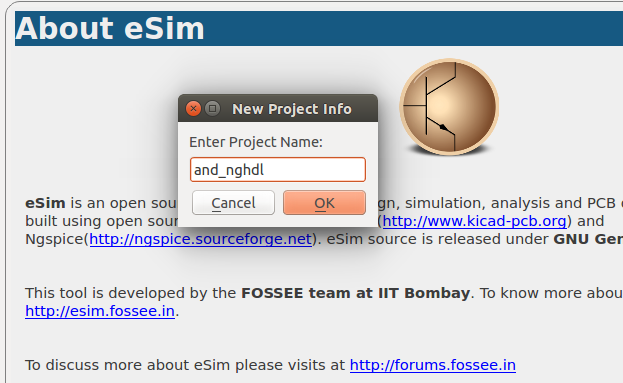
\includegraphics[width = 13cm, height = 7cm]{./NGHDL/screen1.png}
\caption{Creation of a new project}
\label{screen1}
\end{figure}

\item After successful upload of the model using the VHDL code, you can create the schematic of your design by clicking on \texttt{Open Schematic} button on the left pane of the eSim window. Then go to \texttt{Preferences} option on top of the schematic editor window and click on \texttt{Component Libraries} to add the library eSim\_Nghdl.lib in KiCad. Following window will appear as shown in \figref{screen6}, where you will have to click on \textit {Add} button and select the \texttt{eSim\_Nghdl} library. Refer \figref{screen6} and \figref{screen7}. %%last sentence may not be required
    
        \begin{figure}[!htp]
            \centering
            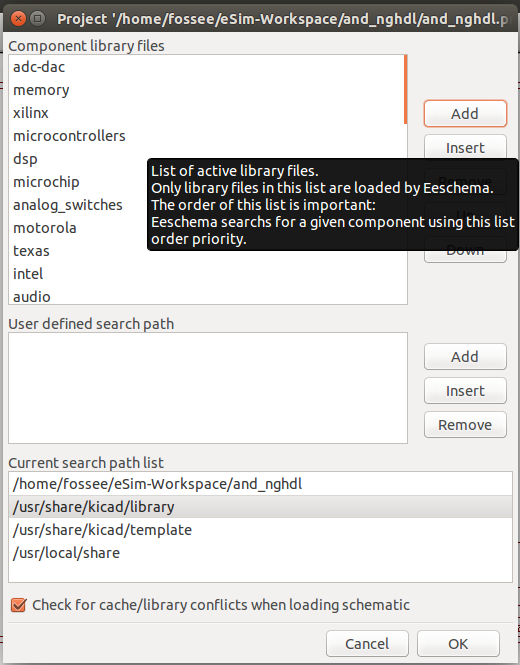
\includegraphics[width =\smfig]{./NGHDL/screen6.png}
            \caption{Adding the digital model library in KiCad}
            \label{screen6}
        \end{figure}


        \begin{figure}[!htp]
            \centering
            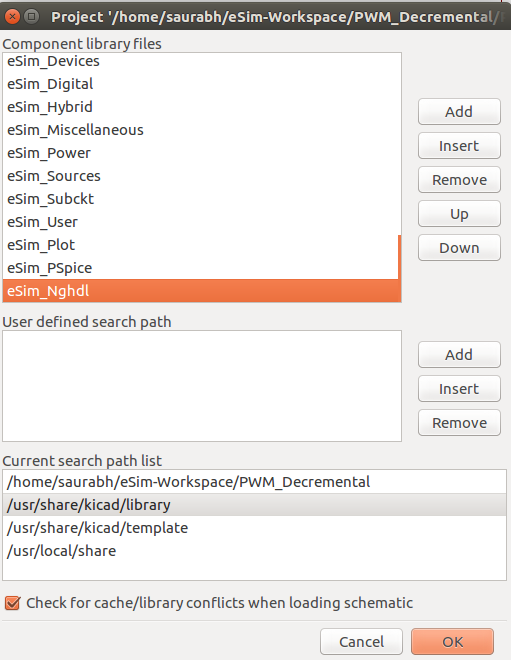
\includegraphics[width =\smfig]{./NGHDL/screen7.png}
            \caption{Selection of library} %%this may not be required either
            \label{screen7}
        \end{figure}


    
    \pagebreak
    \item Next step is to locate the component in \texttt{eSim\_Nghdl} library as shown in \figref{screen9} and place it on the schematic editor as shown in \figref{screen10}.
        \begin{figure}[!htp]
            \centering
            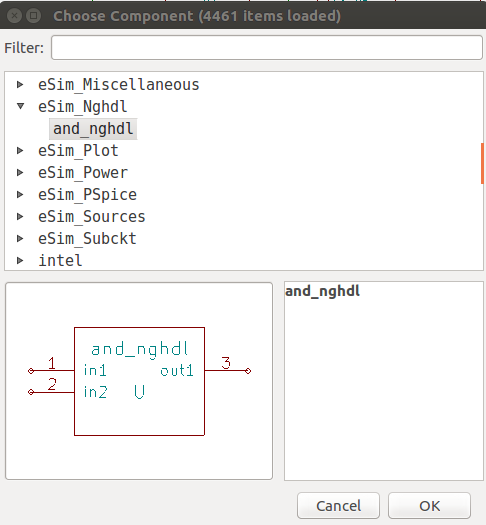
\includegraphics[width =\smfig]{./NGHDL/screen9.png} %%Change this image
            \caption{Locating the component in library} 
            \label{screen9}
        \end{figure}


        \begin{figure}[!htp]
            \centering
            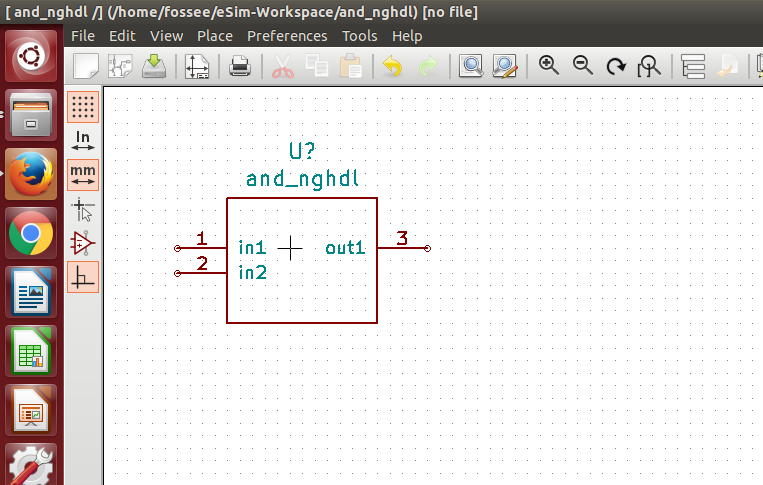
\includegraphics[width =\smfig]{./NGHDL/screen10.png}
            \caption{Placement of component on editor}
            \label{screen10}
        \end{figure}
\pagebreak

\item Now create the schematic as shown in \figref{screen14}, annotate, perform ERC, create the netlist and save the schematic by following the steps given in Chapter 5.
\begin{figure}[!htp]
            \centering
            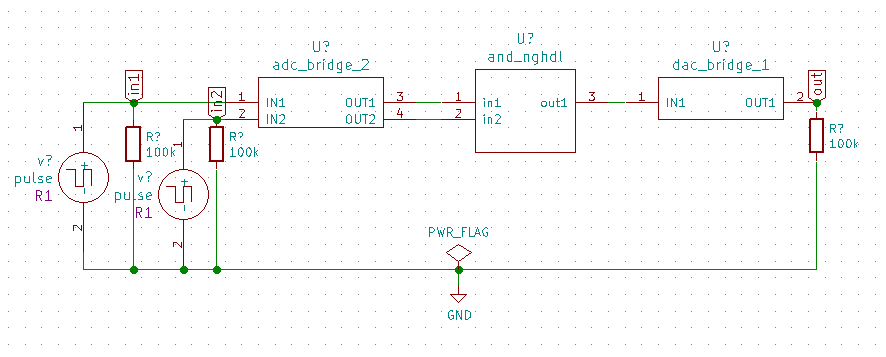
\includegraphics[width =\hgfig]{./NGHDL/screen14.png}
            \caption{Example of an AND gate characteristics circuit}
            \label{screen14}
        \end{figure}

\item After creating the schematic, click on \texttt{KiCad-to-Ngspice converter} and select the type of analysis as transient as shown in \figref{screen15} and set the start, step and stop time as shown in \figref{screen16}
   \begin{figure}[!htp]
                \centering
                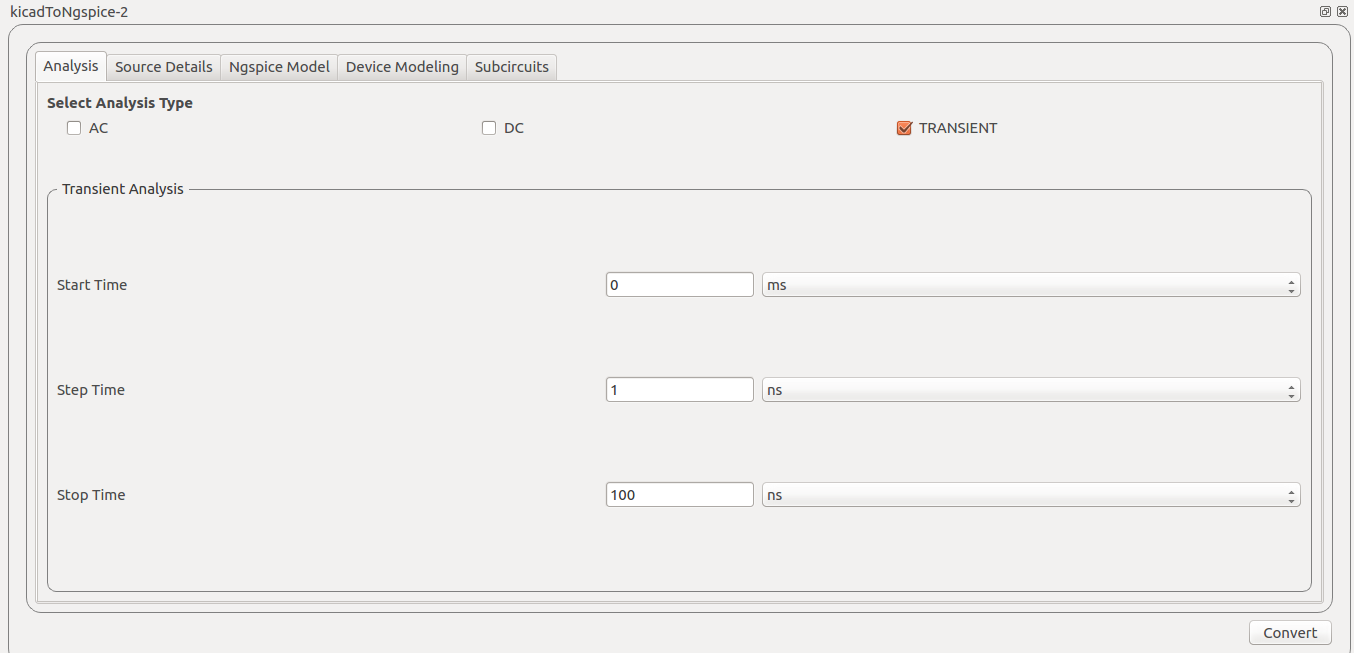
\includegraphics[width =\hgfig]{./NGHDL/screen15.png}
                \caption{Analysis Part I}
                \label{screen15}
            \end{figure}
           \begin{figure}[!htp]
            \centering
            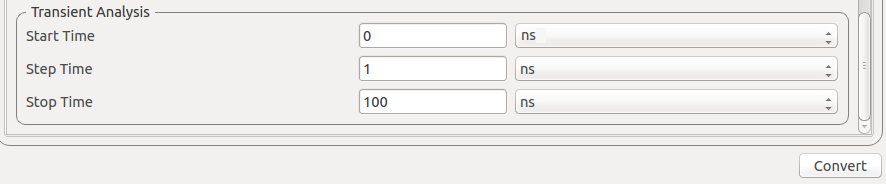
\includegraphics[width =\hgfig]{./NGHDL/screen16.png}
            \caption{Analysis Part II}
            \label{screen16}
        \end{figure}
\pagebreak

\item Now click on \texttt{Source Details} and enter the values for Source v1 and source v2 as shown in figure \figref{val1} and \figref{val2}
\begin{figure}[!htp]
                \centering
                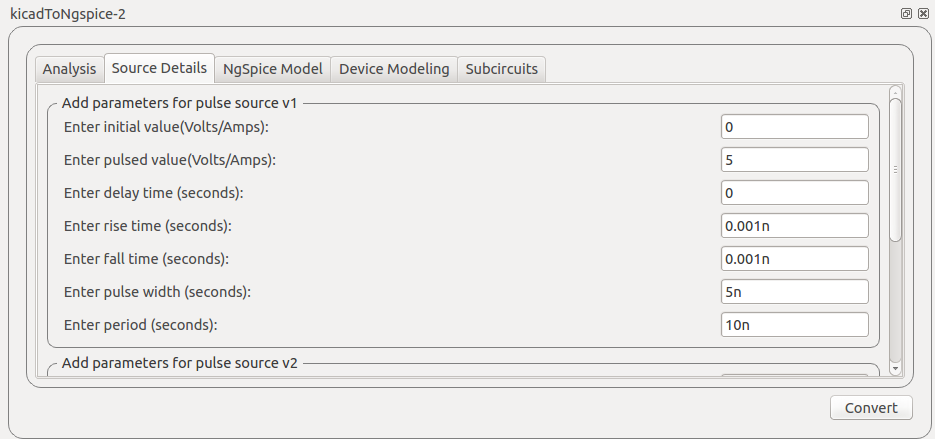
\includegraphics[width =\hgfig]{./NGHDL/val1.png}
                \caption{Value of Source v1}
                \label{val1}
            \end{figure}
           \begin{figure}[!htp]
            \centering
            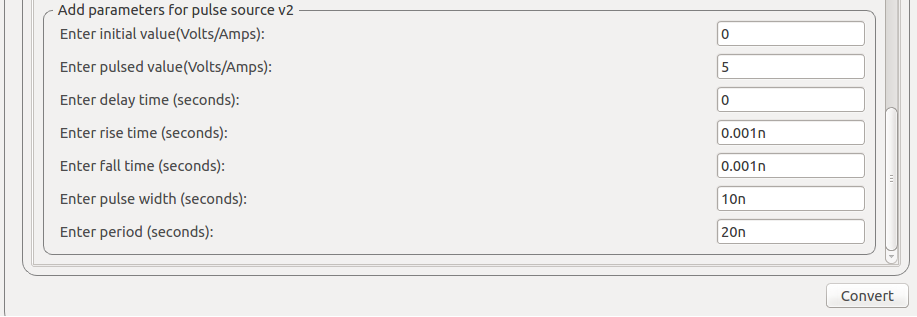
\includegraphics[width =\hgfig]{./NGHDL/val2.png}
            \caption{Value of Source v2}
            \label{val2}
        \end{figure}

\item Now select the option \texttt{Ngspice Model}, window as shown in \figref{screen17} will appear. The values of the parameters listed can be changed per user's requirement. If you have used any semicnductor devices and Subcircuits in your design, then please specify the Spice models and subcircuits in the \texttt{Device Modeling} and \texttt{Subcircuits} tabs of the \texttt{KiCad-to-Ngspice converter} window.  After that click on \texttt{Convert} button. This step will create the simulation compatible netlist.
                    \begin{figure}[!htp]
                        \centering
                        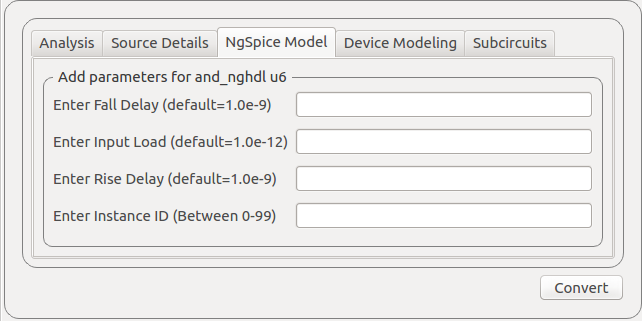
\includegraphics[width =\hgfig]{./NGHDL/screen17.png} %Change the figure
                        \caption{Model Parameters}
                        \label{screen17}
                    \end{figure}
\item Now click on \texttt{Simulation} button, it will display the following windows as shown in \figref{screen19}. This is the Ngspice terminal and Python plot window.
\begin{figure}[!htp]
                        \centering
                        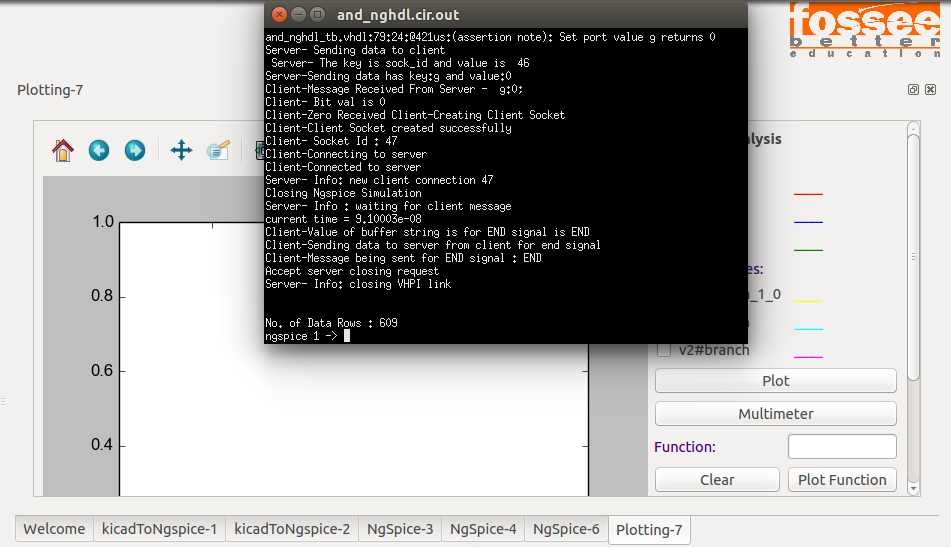
\includegraphics[width =\hgfig]{./NGHDL/screen19.png}
                        \caption{Simulation window}
                        \label{screen19}
                    \end{figure}
\pagebreak 
\item Now select the required nodes and click on \texttt {Plot} button. You can see the plots of input source v1, input source v2 and output as shown in \figref{plotv1}, \figref{plotv2}, and \figref{plotout} respectively.
\begin{figure}[!htp]
                        \centering
                        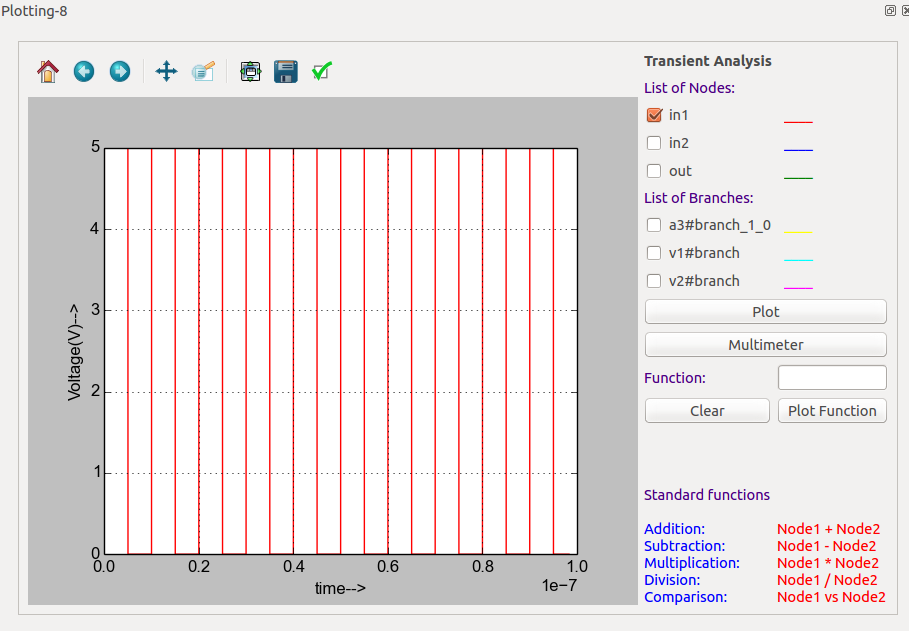
\includegraphics[width =\lgfig]{./NGHDL/plotv1.png}
                        \caption{Plot of Source V1}
                        \label{plotv1}
                    \end{figure}
\begin{figure}[!htp]
                        \centering
                        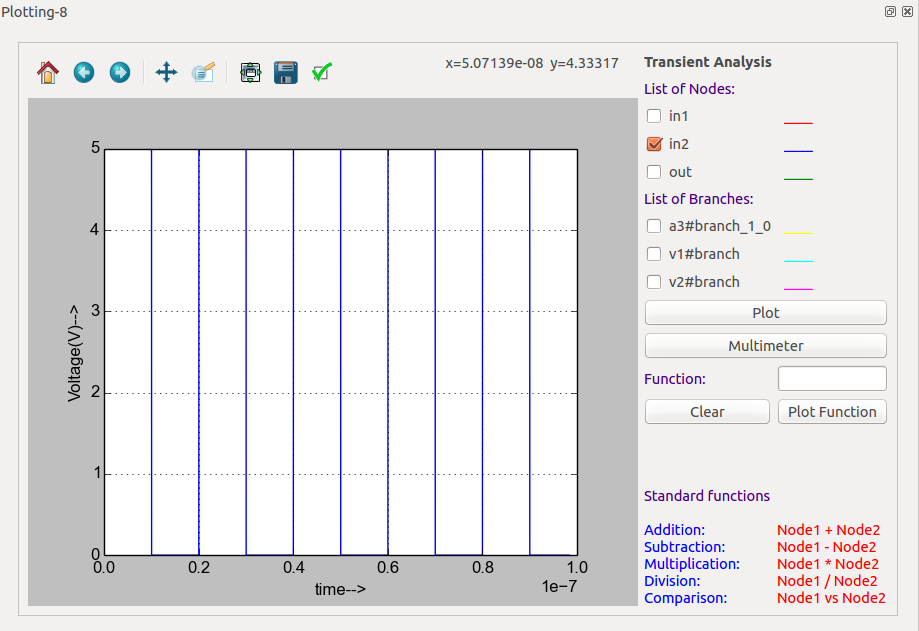
\includegraphics[width =\lgfig]{./NGHDL/plotv2.png}
                        \caption{Plot of source V2}
                        \label{plotv2}
                    \end{figure}
\begin{figure}[!htp]
                        \centering
                        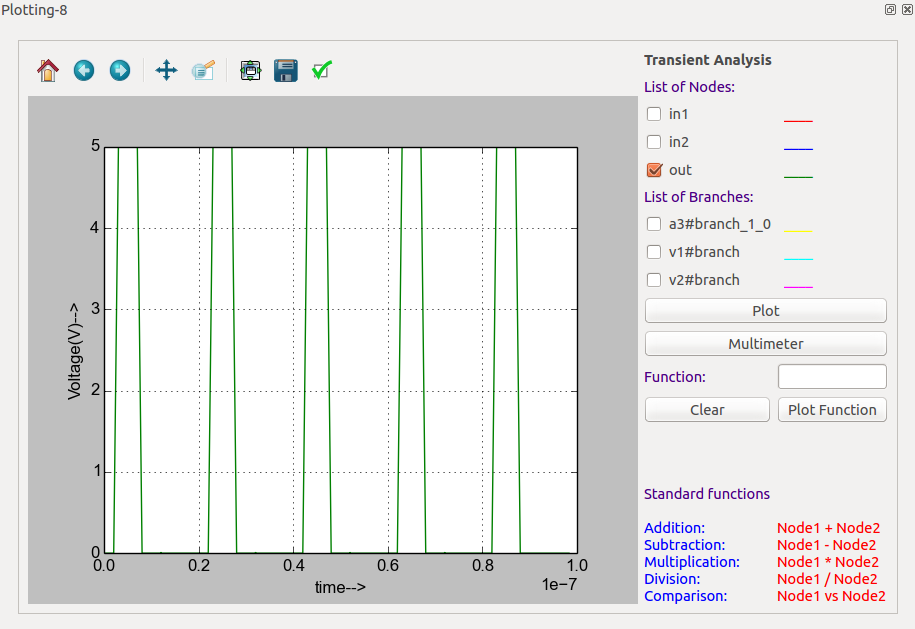
\includegraphics[width =\lgfig]{./NGHDL/plotout.png}
                        \caption{Plot of output}
                        \label{plotout}
                    \end{figure}

        \pagebreak

\end{enumerate}